\documentclass[11pt,a4paper,openany]{ctexbook}
\usepackage[margin=2.2cm,top=2.4cm,bottom=2.35cm]{geometry}
\usepackage{amsmath,amssymb,amsthm,mathtools,bm,siunitx,booktabs,tabularx,array,multirow,longtable}
\usepackage{tikz,pgfplots,tcolorbox,graphicx,float,fancyhdr,hyperref,enumitem,caption,xcolor}
\usetikzlibrary{arrows.meta,calc,positioning,decorations.pathreplacing,patterns,angles,quotes}
\pgfplotsset{compat=1.18}
\hypersetup{colorlinks=true,linkcolor=teal!50!black,urlcolor=teal!60!black}
\definecolor{ink}{HTML}{15384A}
\definecolor{sea}{HTML}{13797B}
\definecolor{gold}{HTML}{9C6B1B}
\definecolor{soft}{HTML}{EEF6F4}
\definecolor{warm}{HTML}{FBF7ED}
\definecolor{lightgray}{HTML}{F6F7F8}
\ctexset{
chapter={format=\Huge\bfseries\color{ink},name={第,章},number=\chinese{chapter}},
section={format=\Large\bfseries\color{sea},name={§},number=\thesection},
subsection={format=\large\bfseries\color{ink}}
}
\setlength{\parindent}{2em}
\setlength{\parskip}{3pt}
\linespread{1.20}

\newcommand{\dd}{\mathrm d}
\newcommand{\ee}{\mathrm e}
\newcommand{\ii}{\mathrm i}
\newcommand{\kb}{k_{\mathrm B}}
\newcommand{\NA}{N_{\mathrm A}}
\newcommand{\pp}[2]{\frac{\partial #1}{\partial #2}}
\newcommand{\avg}[1]{\left\langle #1\right\rangle}
\newcommand{\dif}{\,\mathrm d}
\newcommand{\rev}{\mathrm{rev}}
\newcommand{\const}{\mathrm{const}}
\newcommand{\vu}{\bm{u}}
\newcommand{\vv}{\bm{v}}
\newcommand{\vr}{\bm{r}}

\newtcolorbox{keybox}[1][]{
colback=soft,colframe=sea!70!black,arc=1.2mm,boxrule=.6pt,
title={核心结论},fonttitle=\bfseries,#1}
\newtcolorbox{notebox}[1][]{
colback=warm,colframe=gold!75!black,arc=1.2mm,boxrule=.55pt,
title={理解与辨析},fonttitle=\bfseries,#1}
\newtcolorbox{examplebox}[1][]{
colback=white,colframe=ink!55,arc=1.2mm,boxrule=.55pt,
title={例题与练习},fonttitle=\bfseries,#1}

\pagestyle{fancy}
\fancyhf{}
\fancyhead[LE,RO]{\small\color{sea}普通物理（II）· 热学讲义}
\fancyhead[RE,LO]{\small\leftmark}
\fancyfoot[C]{\thepage}
\setlength{\headheight}{14pt}


\graphicspath{{thermal_source_figs/}}

\begin{document}
\begin{titlepage}
\centering
\vspace*{1.8cm}
{\Large\color{sea}GENERAL PHYSICS II\par}
\vspace{.4cm}
{\fontsize{34}{40}\selectfont\bfseries 普通物理（II）\par}
\vspace{.3cm}
{\LARGE 热学 \par}
\vspace{.8cm}


\begin{tikzpicture}[>=Latex,scale=1.0]
\fill[soft,rounded corners=8pt] (0,0) rectangle (12,5.2);
\draw[ink,thick,->] (1.0,0.8)--(11.0,0.8) node[right] {$V$};
\draw[ink,thick,->] (1.0,0.8)--(1.0,4.6) node[above] {$p$};
\draw[sea,line width=2pt,domain=1.9:9.4,samples=120,smooth] plot (\x,{4.2/(\x-0.7)+0.6});
\draw[gold!90!black,line width=2pt,domain=1.9:9.4,samples=120,smooth] plot (\x,{7.4/((\x-0.7)^1.45)+0.22});
\draw[gray!55,dashed] (2.15,4.05) -- (9.0,1.02);
\node[fill=white,rounded corners=2pt,text=sea] at (7.9,2.7) {状态方程};
\node[fill=white,rounded corners=2pt,text=gold!80!black] at (7.2,3.8) {气体动理论与统计规律};
\foreach \x/\y in {2.2/4.0,3.2/2.8,4.7/2.1,6.7/1.64,8.7/1.35}
  {\fill[sea] (\x,\y) circle(1.7pt);}
\end{tikzpicture}

\vfill
\begin{minipage}{.88\textwidth}
\small
\textbf{编制原则}\quad
本讲义基于课堂纯板书整理，由大语言模型辅助转录与排版。内容可能存在公式偏差或疏漏，请以官方教材及课堂原话为准。仅供学习交流，未经许可请勿用于商业用途。
\end{minipage}

\vfill
{\small 适用对象：已学高中概率、微积分和普通物理力学的读者\hfill \today\par}
\end{titlepage}

\frontmatter 
\tableofcontents 


\mainmatter 

\chapter{热力学系统的平衡态及状态方程}

\section{热力学系统与平衡态}
热力学研究由大量微观粒子组成的宏观系统的共同规律。研究时首先选取一个\textbf{系统}（system），其余部分称为\textbf{外界}（surroundings），两者之间由真实或假想的边界区分。

按照系统与外界之间是否交换物质和能量，常把系统分为：
\begin{itemize}[leftmargin=2.2em]
\item \textbf{开系统}：与外界既能交换物质，也能交换能量；
\item \textbf{封闭系统}：与外界不交换物质，但可交换能量；
\item \textbf{孤立系统}：与外界既不交换物质，也不交换能量。
\end{itemize}

研究热学时最基本的宏观量包括：
\[
V\ (\text{体积}),\qquad m\ (\text{质量}),\qquad 
N=\frac{m}{m_0}\ (\text{分子数}),\qquad
\nu=\frac{N}{\NA}\ (\text{物质的量}),
\]
\[
p\ (\text{压强}),\qquad T\ (\text{温度}).
\]
其中 $\NA=6.022\times10^{23}\,\mathrm{mol^{-1}}$ 是阿伏伽德罗常数。

温度 $T$ 是热学中特别重要的状态量。若系统处于平衡态，则宏观量随时间不变，此时系统可以用一组确定的状态参量来描述。

\subsection*{平衡态与稳态}
\textbf{平衡态}是指：在没有外界额外驱动的情况下，系统内各处宏观量不随时间变化，也不存在持续的宏观流。平衡通常包含热平衡、力学平衡和化学平衡。

\textbf{稳态}是指：虽然系统可能仍有外界驱动，但宏观量随时间不再变化。稳态不一定是平衡态，例如两端保持定温差时的导热棒中有持续热流，这是一种稳态，但不是平衡态。

\begin{notebox}
注意：\textbf{准静态过程不等于可逆过程}。准静态仅表示过程足够慢，使系统始终可近似视为经过一系列平衡态；可逆过程还要求没有摩擦、黏滞、有限温差传热等耗散因素。
\end{notebox}

对于由若干互不相互作用的子系统组成的整体，有些状态量可加，有些不可加。若总量等于各子系统量的代数和，则称该量为\textbf{广延量}；否则称其为\textbf{强度量}。例如
\[
N=\sum_i N_i,\qquad \nu=\sum_i \nu_i,\qquad V=\sum_i V_i
\]
是广延量，而温度 $T$ 与压强 $p$ 一般不是简单相加的。

\begin{keybox}
广延量：$N,\nu,V,m,U,S,\cdots$；\qquad
强度量：$T,p,\rho,\cdots$。
\end{keybox}

\section{温度、温标与热力学第零定律}
热力学第零定律是温度概念的基础：如果系统 $A$ 与系统 $C$ 处于热平衡，系统 $B$ 与系统 $C$ 也处于热平衡，那么 $A$ 与 $B$ 也处于热平衡。于是我们可以引入一个状态量来刻画系统“冷热”的程度，这个状态量就是温度。

\subsection*{经验温标}
历史上常见的经验温标有摄氏温标和华氏温标：
\[
t_{F}=32+\frac95t_C .
\]
摄氏温标把标准大气压下冰水混合物的温度记为 $0^\circ\mathrm C$，水沸腾的温度记为 $100^\circ\mathrm C$。

\subsection*{热力学温标与理想气体温标}
热力学温标以开尔文（Kelvin, K）为单位。对于理想气体，可以在低压极限用压强或体积定义温标。若把水的三相点温度定为 $273.16\,\mathrm K$，则在体积固定时可取
\[
T(p)=273.16\lim_{p_{\mathrm{triple}}\to0}\frac{p}{p_{\mathrm{triple}}},
\]
在压强固定时可取
\[
T(V)=273.16\lim_{V_{\mathrm{triple}}\to0}\frac{V}{V_{\mathrm{triple}}}.
\]
现代 SI 中，开尔文的定义等价于固定玻尔兹曼常数的数值；理想气体温标可视为其物理实现方式之一。摄氏温标与热力学温标的关系是
\[
T=t_C+273.15 .
\]

\section{状态方程}
一定量的简单可压缩平衡系统，通常可用压强 $p$、体积 $V$、温度 $T$ 之间的关系来描述。一般写成
\[
f(p,V,T)=0.
\]
由于三个量中只有两个是独立的，所以只要确定其中两个量，第三个量就被状态方程确定。

\subsection*{三个响应系数}
重点引入了三个常用的宏观响应系数：
\[
\alpha\equiv \frac1V\left(\pp VT\right)_p
\qquad \text{（体膨胀系数）},
\]
\[
\beta\equiv \frac1p\left(\pp pT\right)_V
\qquad \text{（等体压温系数）},
\]
\[
\kappa_T\equiv -\frac1V\left(\pp Vp\right)_T
\qquad \text{（等温压缩系数）}.
\]
这里负号的意义是：通常情况下，在温度不变时压强增大，体积减小，所以 $\left(\partial V/\partial p\right)_T<0$，加入负号后压缩系数为正。

\subsection*{恒等式 $\alpha=p\beta\kappa_T$ 的推导}
由状态方程 $f(p,V,T)=0$，全微分得
\[
\pp fp\dd p+\pp fV\dd V+\pp fT\dd T=0.
\]
分三种情形讨论：

\paragraph{1. 固定 $p$} 令 $\dd p=0$，则
\[
\pp fV \dd V+\pp fT \dd T=0
\quad\Longrightarrow\quad
\left(\pp VT\right)_p=-\frac{(\partial f/\partial T)}{(\partial f/\partial V)}.
\]
于是
\[
\alpha=-\frac1V\frac{f_T}{f_V}.
\]

\paragraph{2. 固定 $V$} 令 $\dd V=0$，则
\[
\pp fp \dd p+\pp fT \dd T=0
\quad\Longrightarrow\quad
\left(\pp pT\right)_V=-\frac{f_T}{f_p}.
\]
于是
\[
\beta=-\frac1p\frac{f_T}{f_p}.
\]

\paragraph{3. 固定 $T$} 令 $\dd T=0$，则
\[
\pp fp \dd p+\pp fV \dd V=0
\quad\Longrightarrow\quad
\left(\pp Vp\right)_T=-\frac{f_p}{f_V}.
\]
于是
\[
\kappa_T=\frac1V\frac{f_p}{f_V}.
\]

三式相乘即可得
\[
p\beta\kappa_T
=
p\left(-\frac1p\frac{f_T}{f_p}\right)
\left(\frac1V\frac{f_p}{f_V}\right)
=
-\frac1V\frac{f_T}{f_V}
=\alpha.
\]
故
\[
\boxed{\alpha=p\beta\kappa_T}.
\]

\subsection*{理想气体状态方程}
在本节给出了理想气体的状态方程
\[
\boxed{pV=\nu RT=Nk_{\mathrm B}T},
\]
其中
\[
R=8.31\,\mathrm{J/(mol\cdot K)}
\]
是摩尔气体常数，满足
\[
R=\NA \kb .
\]

如果写成粒子数密度 $n=N/V$ 的形式，则
\[
p=n\kb T.
\]

对于理想气体，由状态方程可直接算得：
\[
\alpha=\frac1T,\qquad
\beta=\frac1T,\qquad
\kappa_T=\frac1p.
\]

\subsection*{Dalton 分压定律}
若几种理想气体在同一温度下混合，且它们彼此近似不相互作用，则总压强等于各组分在该体积中单独存在时所产生压强之和：
\[
\boxed{p=\sum_i p_i}.
\]
这就是 Dalton 分压定律。


\subsection*{例题：连通球泡的温度与压强}
设上端球泡 $A$ 与下端球泡 $B$ 由细管相连，$A$ 保持温度 $T_A$，$B$ 的温度待求，两球泡内气体初始压强为 $p_0$，总体积的变化通过后续的操作体现。以下保留使用的\emph{两状态理想气体方程}：应分别列写
\[
p_0V_A=\nu_A RT_A,\qquad p_0V_B=\nu_B RT_B
\]
以及操作后的
\[
pV_A=\nu_A'RT_A,\qquad pV_B=\nu_B'RT_B',\qquad
\nu_A+\nu_B=\nu_A'+\nu_B'.
\]
在讨论的“球泡 $B$ 温度由 $T_0$ 变为 $T$”的具体设定下，
若 $A$ 温度 $T_0$ 保持不变，气体始终连通并在各状态下有共同压强，则
\[
\frac{p_0(V_A+V_B)}{RT_0}
=\frac{pV_A}{RT_0}+\frac{pV_B}{RT}.
\]
因此
\[
\boxed{T=\frac{pV_BT_0}{p_0(V_A+V_B)-pV_A}.}
\]
该式清楚表明：不能在这类题中把两球泡物质的量分别看成不变，它们通过细管交换粒子。


\begin{notebox}
这里的“初态两球泡都在 $T_0$”是为了写出的压强--体积形式；若原题使用两个不同初温，应返回最一般的粒子数守恒式，不能直接套用该简化结果。
\end{notebox}

\begin{figure}[htbp]\centering
\begin{tikzpicture}[>=Latex,scale=.9]
\draw[ink,thick] (1,3.1) circle(.62) (1,-.4) ellipse(.44 and .62);
\draw[ink,thick] (.89,2.49)--(.89,.23) (1.11,2.49)--(1.11,.23);
\draw[->,sea,thick] (1,3.1)--(1,3.47);
\node[right] at (1.72,3.12) {$A:\ V_A,\ T_0$};
\node[right] at (1.5,-.42) {$B:\ V_B,\ T$};
\node[right,align=left] at (4.3,1.4) {导热细管连通\\两室压强相同；气体可以交换};
\end{tikzpicture}
\caption{连通双球泡气体温度计：$A$ 保持室温，$B$ 接触待测物质。}
\end{figure}

\subsection*{Van der Waals 状态方程}
为了修正理想气体模型忽略分子体积和分子间作用的不足，引入了 Van der Waals 方程
\[
\boxed{\left(p+\frac{a\nu^2}{V^2}\right)(V-\nu b)=\nu RT}.
\]
这里 $a$ 用来描述分子间吸引作用的平均修正，$b$ 描述分子有限体积造成的可利用空间修正。该方程能定性解释实际气体在低温下出现液化和相变的趋势。


\subsection*{Van der Waals 方程的响应系数计算}
用\emph{粒子数密度} $n=N/V$ 表示时，可写为
\[
p=\frac{n\kb T}{1-bn}-an^2
\]
（此处 $a,b$ 是与 $n$ 定义相匹配的参数，勿与按摩尔体积书写的系数混用）。
固定 $N$ 时 $n=N/V$，所以
\[
\left(\frac{\partial p}{\partial T}\right)_V
=\frac{n\kb}{1-bn},
\quad
\left(\frac{\partial p}{\partial V}\right)_T
=-\frac nV\left[\frac{\kb T}{(1-bn)^2}-2an\right].
\]
用 $f=p-p(V,T)=0$ 的偏导关系计算体膨胀系数：
\[
\alpha=-\frac1V
\frac{(\partial p/\partial T)_V}{(\partial p/\partial V)_T}
=\boxed{\frac{\kb/(1-bn)}
{\kb T/(1-bn)^2-2an}}.
\]
还尝试通过两端微分直接算出这一结构；正确结果必须满足稀薄极限 $n\to0$ 时 $\alpha\to1/T$。

\section{理想气体微观模型}
从分子运动角度可以推导气体压强公式。

\subsection*{模型假设}
理想气体的微观模型包含以下基本假设：
\begin{enumerate}[leftmargin=2.3em]
\item 气体由大量完全相同的分子组成，分子可看成质点；
\item 分子做无规则热运动；
\item 除碰撞外，分子之间无相互作用；
\item 分子与容器壁以及分子之间的碰撞都是弹性的；
\item 在平衡态下，速度分布各向同性。
\end{enumerate}

\subsection*{压强公式的一维推导}
考虑边长为 $L$ 的立方体容器。设某一分子的 $x$ 分速度为 $v_x$，它每次撞击与 $x$ 轴垂直的墙面时，给予墙的冲量大小为
\[
\Delta p_x=2mv_x.
\]
相邻两次撞击同一墙面的时间间隔为
\[
\Delta t=\frac{2L}{|v_x|}.
\]
因此该分子对该墙的平均作用力为
\[
F_x=\frac{\Delta p_x}{\Delta t}=\frac{mv_x^2}{L}.
\]
容器壁面积为 $A=L^2$，体积为 $V=L^3$，于是所有分子对墙的总压强为
\[
p=\frac1A\sum_i\frac{mv_{ix}^2}{L}
=\frac1V\sum_i mv_{ix}^2
=nm\avg{v_x^2},
\]
其中 $n=N/V$ 是数密度。

由于平衡态下各向同性，
\[
\avg{v_x^2}=\avg{v_y^2}=\avg{v_z^2}
=\frac13\avg{v^2}.
\]
因此
\[
\boxed{p=\frac13nm\avg{v^2}}.
\]


\subsection*{球坐标积分版的压强推导}
设数密度为 $n$，速率概率密度为 $f_v(v)$，各向同性分布。取面积 $A$ 的壁面，定义速度与壁面内法线夹角为 $\theta\in[0,\pi/2]$。
时间 $\Delta t$ 内撞壁分子的来源柱体积为 $Av\cos\theta\Delta t$，
落在速率区间 $[v,v+\dd v]$ 和立体角
$\dd\Omega=\sin\theta\dd\theta\dd\phi$ 内的粒子数为
\[
\dd N=nAv\cos\theta\Delta t\;
f_v(v)\dd v\,\frac{\sin\theta\dd\theta\dd\phi}{4\pi}.
\]
一个分子法向动量改变 $2mv\cos\theta$，所以总冲量
\[
\begin{aligned}
\Delta P
=&\int_0^\infty\int_0^{2\pi}\int_0^{\pi/2}
2mv\cos\theta\;\dd N\\
=&\frac{nmA\Delta t}{2\pi}
\int_0^\infty f_v(v)v^2\dd v
\int_0^{2\pi}\dd\phi
\int_0^{\pi/2}\cos^2\theta\sin\theta\dd\theta.
\end{aligned}
\]
角积分为 $2\pi$ 与 $1/3$，从而
\[
\boxed{p=\frac{\Delta P}{A\Delta t}=\frac13nm\avg{v^2}.}
\]
它还解释了为什么流出小孔的分子束应带有方向权重 $\cos\theta$。

\subsection*{与温度的联系}
把上式与理想气体状态方程
\[
p=n\kb T
\]
对比，得到
\[
\frac13nm\avg{v^2}=n\kb T
\quad\Longrightarrow\quad
\boxed{\frac12m\avg{v^2}=\frac32\kb T}.
\]
即：\textbf{温度与分子平均平动动能成正比}。

\begin{notebox}
这一定律非常重要。它说明温度并不是单个分子的速度，而是大量分子热运动平均动能的宏观表征。后文 Maxwell 分布和能量均分定理都要用到这一关系。
\end{notebox}

%===========================
\chapter{热平衡态的统计分布规律}

\section{概率与统计预备知识}
在进入统计物理的推导前，我们需要一些基本的概率论工具。本节将相关概率知识统一放在这里，供后文使用。

\subsection*{离散概率与连续概率密度}
对离散随机变量 $X$，有
\[
\sum_i P(X=x_i)=1.
\]
对连续随机变量，通常用\textbf{概率密度函数} $f(x)$ 描述：
\[
P(a\le X\le b)=\int_a^b f(x)\dd x,\qquad
f(x)\ge0,\qquad
\int_{-\infty}^{\infty}f(x)\dd x=1.
\]
注意：对于连续随机变量，恰好取到一个精确值的概率一般为零，即 $P(X=x_0)=0$。

\subsection*{平均值、方差与均方根}
随机变量的平均值（期望）定义为
\[
\avg X=\sum_i x_i p_i
\quad \text{或}\quad
\avg X=\int_{-\infty}^\infty x f(x)\dd x.
\]
方差与均方根分别为
\[
\mathrm{Var}(X)=\avg{(X-\avg X)^2}
=\avg{X^2}-\avg X^2,
\qquad
X_{\mathrm{rms}}=\sqrt{\avg{X^2}}.
\]
后文中的方均根速率 $v_{\mathrm{rms}}$ 就是这一概念在速度问题中的应用。

\subsection*{独立性和条件概率}
若随机变量 $X,Y$ 独立，则联合概率密度可分解为
\[
f_{X,Y}(x,y)=f_X(x)f_Y(y).
\]
对事件 $A,B$，条件概率满足
\[
P(A|B)=\frac{P(A\cap B)}{P(B)}\qquad (P(B)\neq0).
\]
Maxwell 分布的推导要用到速度三个分量相互独立且分布形式相同的思想。

\subsection*{常用积分}
后文将频繁用到如下高斯积分：
\[
\int_{-\infty}^{\infty}\ee^{-ax^2}\dd x
=
\sqrt{\frac{\pi}{a}}
\qquad (a>0),
\]
以及
\[
\int_0^\infty x^2\ee^{-ax^2}\dd x
=
\frac{\sqrt{\pi}}{4a^{3/2}},
\qquad
\int_0^\infty x^3\ee^{-ax^2}\dd x
=
\frac{1}{2a^2}.
\]

\begin{keybox}
使用下面的基本工具即可掌握：\textbf{归一化}、\textbf{平均值}、\textbf{方差}、\textbf{独立性}以及\textbf{高斯积分}。这些工具足以应付普通物理层次的 Maxwell 分布、自由程分布和布朗运动的计算。
\end{keybox}

\section{Maxwell 分布与 Maxwell--Boltzmann 分布律}
先从平衡气体中的三维速度分布出发，推导速率分布与三种典型速率；然后通过速率选择实验引出泄流数率，结合三个应用例子，最终把速度统计推广到外力场中的空间分布。

\subsection*{三维速度分布函数}
记平衡态下分子的速度分布函数为
\[
f(v_x,v_y,v_z),
\]
其含义是：速度分量分别落在区间
\[
[v_x,v_x+\dd v_x],\quad [v_y,v_y+\dd v_y],\quad [v_z,v_z+\dd v_z]
\]
内的分子所占概率为
\[
f(v_x,v_y,v_z)\dd v_x\dd v_y\dd v_z.
\]
归一化条件是
\[
\iiint_{-\infty}^{\infty}
f(v_x,v_y,v_z)\dd v_x\dd v_y\dd v_z=1.
\]

\subsection*{推导 Maxwell 速度分布}
推导使用三个基本假设：

\begin{enumerate}[leftmargin=2.3em]
\item 平衡态下速度分布与时间无关；
\item 空间中没有优先方向，分布具有\textbf{各向同性}；
\item 三个速度分量相互独立，且服从相同的分布。
\end{enumerate}

由独立性，
\[
f(v_x,v_y,v_z)=f_x(v_x)f_y(v_y)f_z(v_z).
\]
由各向同性，分布只能依赖于
\[
v^2=v_x^2+v_y^2+v_z^2,
\]
即
\[
f(v_x,v_y,v_z)=\Phi(v_x^2+v_y^2+v_z^2).
\]
于是
\[
\ln f_x(v_x)+\ln f_y(v_y)+\ln f_z(v_z)
=
\ln \Phi(v_x^2+v_y^2+v_z^2).
\]
对 $v_x$ 求偏导：
\[
\frac{f_x'(v_x)}{f_x(v_x)}
=
2v_x\frac{\Phi'(v^2)}{\Phi(v^2)}.
\]
左边只依赖于 $v_x$，右边若要对任意 $v_y,v_z$ 都成立，必须有
\[
\frac{\Phi'(v^2)}{\Phi(v^2)}=-a
\]
为常数。于是
\[
\Phi(v^2)=Ce^{-av^2}.
\]
从而
\[
f(v_x,v_y,v_z)=Ce^{-a(v_x^2+v_y^2+v_z^2)}.
\]

下面利用归一化条件和平均动能关系来确定常数 $C$ 和参数 $a$。

由高斯积分，
\[
1=\iiint f\dd v_x\dd v_y\dd v_z
=
C\left(\int_{-\infty}^{\infty}e^{-av_x^2}\dd v_x\right)^3
=
C\left(\sqrt{\frac{\pi}{a}}\right)^3,
\]
因此
\[
C=\left(\frac{a}{\pi}\right)^{3/2}.
\]
故
\[
f(v_x,v_y,v_z)=\left(\frac{a}{\pi}\right)^{3/2}
e^{-a(v_x^2+v_y^2+v_z^2)}.
\]

再利用
\[
\frac12m\avg{v^2}=\frac32\kb T.
\]
由分布可算得
\[
\avg{v_x^2}=\frac{1}{2a},
\qquad
\avg{v^2}=3\avg{v_x^2}=\frac{3}{2a}.
\]
于是
\[
\frac12m\cdot\frac{3}{2a}=\frac32\kb T
\quad\Longrightarrow\quad
a=\frac{m}{2\kb T}.
\]

最终得到 Maxwell 三维速度分布：
\[
\boxed{
f(v_x,v_y,v_z)=
\left(\frac{m}{2\pi\kb T}\right)^{3/2}
\exp\!\left[-\frac{m(v_x^2+v_y^2+v_z^2)}{2\kb T}\right]
}.
\]

\subsection*{速度分量分布}
由三维分布可知任一方向上的速度分量都服从正态分布：
\[
f_x(v_x)=
\sqrt{\frac{m}{2\pi\kb T}}
\exp\!\left(-\frac{mv_x^2}{2\kb T}\right),
\]
$y,z$ 方向同理。它们的均值为零，方差为
\[
\avg{v_x^2}=\frac{\kb T}{m}.
\]

\subsection*{速率分布函数}
速率是
\[
v=\sqrt{v_x^2+v_y^2+v_z^2}.
\]
速度空间中速率位于 $[v,v+\dd v]$ 的点构成一个半径为 $v$、厚度为 $\dd v$ 的球壳，其体积为
\[
4\pi v^2\dd v.
\]
因此速率分布函数为
\[
f_v(v)\dd v
=
4\pi v^2
\left(\frac{m}{2\pi\kb T}\right)^{3/2}
\exp\left(-\frac{mv^2}{2\kb T}\right)\dd v.
\]
即
\[
\boxed{
f_v(v)=4\pi
\left(\frac{m}{2\pi\kb T}\right)^{3/2}
v^2
\exp\left(-\frac{mv^2}{2\kb T}\right)
}\qquad (v\ge0).
\]

\begin{center}
\begin{tikzpicture}
\begin{axis}[width=.82\textwidth,height=6.1cm,
xlabel={速率的无量纲变量 $x=v/\sqrt{2\kb T/m}$},
ylabel={$f_x(x)$},
xmin=0,xmax=3.5,ymin=0,ymax=.9,
grid=major,grid style={gray!18},
axis lines=left,tick label style={font=\small}]
\addplot[sea,very thick,domain=0:3.5,samples=200]{4/sqrt(pi)*x^2*exp(-x^2)};
\addplot[gold!85!black,dashed,thick] coordinates {(1,0) (1,0.83)};
\node[anchor=south west,font=\small] at (axis cs:1.03,0.73) {最概然速率};
\end{axis}
\end{tikzpicture}
\captionof{figure}{Maxwell 速率分布函数的形状。}
\end{center}

\subsection*{三种典型速率}
注意：最概然速率、平均速率和方均根速率\textbf{不是同一个量}。

\paragraph{1. 最概然速率}
由
\[
\frac{\dd f_v}{\dd v}=0
\]
求极大值点。等价地，求
更直接地，令
\[
\frac{\dd}{\dd v}\left(v^2e^{-mv^2/(2\kb T)}\right)=0.
\]
得到
\[
\boxed{v_{\mathrm{mp}}=\sqrt{\frac{2\kb T}{m}}}.
\]

\paragraph{2. 平均速率}
\[
\avg v=\int_0^\infty vf_v(v)\dd v
=
\boxed{\sqrt{\frac{8\kb T}{\pi m}}}.
\]

\paragraph{3. 方均根速率}
\[
v_{\mathrm{rms}}=\sqrt{\avg{v^2}}
=
\sqrt{\int_0^\infty v^2f_v(v)\dd v}
=
\boxed{\sqrt{\frac{3\kb T}{m}}}.
\]

三者满足
\[
v_{\mathrm{mp}}<\avg v<v_{\mathrm{rms}}.
\]

\begin{notebox}
需要注意：最概然速率对应的是\textbf{速率分布}的峰值，而不是三维速度分布或某个速度分量分布的峰值。三维速度分布在 $\vv=\bm0$ 处达到最大，但速率分布在 $v=0$ 处反而为零，因为速度空间球壳体积因子 $4\pi v^2$ 在起作用。
\end{notebox}

\subsection*{温度对分布的影响}
温度升高时，分布曲线展宽，峰值右移且变低。这意味着高温时分子更倾向于出现较大速率。



\subsection*{Miller--Kusch 速率选择实验：仪器实际测量什么？}
Maxwell 速率分布描述的是\emph{在气体内部随机选取一个分子}时的速率统计。实验上无法逐个观察容器中的全部分子，Miller--Kusch 实验因而先让金属原子从热源的小孔逸出，形成准直分子束，再以旋转的狭缝选择速率，最后在探测器中计数。

选择器中两个通道位置在传播方向相距 $L$、方位角错开 $\Delta\theta$。若选择器以角速度 $\omega$ 转动，速率为 $v$ 的粒子飞过距离 $L$ 需要时间 $L/v$。要通过前后两个狭缝，必须近似满足
\[
\omega\frac{L}{v}=\Delta\theta
\qquad\Longrightarrow\qquad
\boxed{v\simeq\frac{\omega L}{\Delta\theta}}.
\]
对于周期性狭缝还可能出现附加的周期透过条件；上式只描述选定的一条主透过支路。

\begin{figure}[htbp]\centering
\begin{tikzpicture}[>=Latex,scale=.88]
\fill[gold!12,rounded corners=5pt] (-.7,-.48) rectangle (1.4,.62);
\draw[ink,thick] (0.1,.08) circle(.30);
\foreach \k in {0,...,5} {
 \pgfmathsetmacro{\ang}{\k*60}
 \fill[gold!85!black] ({.1+.19*cos(\ang)},{.08+.19*sin(\ang)}) circle(1pt);
}
\node[below] at (.15,-.55) {热原子源};
\draw[ink,thick] (2.2,-.5)--(2.2,-.08) (2.2,.18)--(2.2,.6);
\node[below] at (2.2,-.55) {准直孔};
\draw[sea,thick,rounded corners=2pt] (3.2,-.42) rectangle (6.5,.55);
\draw[ink,line width=1.4pt] (3.45,-.42)--(3.45,-.09) (3.45,.13)--(3.45,.55);
\draw[ink,line width=1.4pt] (6.2,-.42)--(6.2,-.09) (6.2,.13)--(6.2,.55);
\draw[->,gold!85!black,thick] (3.8,.72) arc[start angle=130,end angle=-70,radius=.32];
\node[above] at (4.92,.55) {旋转选择器 $\omega$};
\draw[<->,ink] (3.45,-.76)--(6.2,-.76) node[midway,below] {$L$};
\draw[->,sea,ultra thick] (.5,.025)--(7.3,.025);
\draw[ink,thick,fill=soft] (7.4,-.42) rectangle (8.5,.49);
\node[below] at (7.95,-.53) {探测器};
\end{tikzpicture}
\caption{速率选择实验的原理示意：旋转狭缝将分子的飞行时间转换为速率选择条件。}
\end{figure}

\textbf{一个必须区分的问题：}探测器记录的是\emph{单位时间穿过小孔、选择器并到达探测器的粒子数}，而不是容器内部随机抽取分子的概率。因此在把实验计数与 Maxwell 分布比较之前，必须先计算\textbf{小孔泄流的分子数率}，再考虑选择器的透过率与探测效率。接下来先在小孔理想、选择器尚未筛选速率的情况下完成这一步。

\subsection*{小孔泄流数率与泄流分子通量}
设气体在容器内保持温度 $T$、数密度 $n$，壁上有面积为 $A$ 的极小薄孔，孔外足够稀薄。孔尺寸需小于分子平均自由程，使孔内碰撞可以忽略，且气体在孔内侧仍近似满足 Maxwell 分布。考虑速率 $v$、速度方向与孔外法线夹角 $\theta$ 的分子。时间 $\Delta t$ 内能穿过小孔的分子起源于体积
\[
\dd V=A v\cos\theta\,\Delta t,\qquad 0\le\theta\le\frac{\pi}{2}.
\]
由于方向各向同性，立体角概率元为
\[
\frac{\dd\Omega}{4\pi}
=\frac{\sin\theta\,\dd\theta\,\dd\varphi}{4\pi}.
\]
于是速率属于 $[v,v+\dd v]$ 的穿孔分子数为
\[
\begin{aligned}
\dd N(v)
&=nA\Delta t\,v f_v(v)\dd v
\int_0^{2\pi}\!\!\int_0^{\pi/2}
\cos\theta\,\frac{\sin\theta\,\dd\theta\,\dd\varphi}{4\pi}\\
&=\frac14 nA\Delta t\,v f_v(v)\dd v,
\end{aligned}
\]
这里使用了
\[
\int_0^{2\pi}\dd\varphi=2\pi,\qquad
\int_0^{\pi/2}\sin\theta\cos\theta\,\dd\theta=\frac12.
\]
对全部速率积分：
\[
\Delta N=\frac14nA\Delta t\int_0^\infty vf_v(v)\dd v
=\frac14nA\bar v\,\Delta t.
\]
因此，\textbf{单位时间穿过整个小孔的分子数率}和\textbf{单位面积、单位时间的泄流数率}分别是
\[
\boxed{\dot N=\frac{\Delta N}{\Delta t}=\frac14nA\bar v},
\qquad
\boxed{\Gamma=\frac{\dot N}{A}=\frac14n\bar v}.
\]
由 Maxwell 分布的平均速率
$\bar v=\sqrt{8\kb T/(\pi m)}$ 和 $p=n\kb T$，还可写作
\[
\Gamma=\frac{p}{\sqrt{2\pi m\kb T}},\qquad
\dot N=\frac{pA}{\sqrt{2\pi m\kb T}}.
\]
$\dot N$ 的量纲是 $\mathrm{s^{-1}}$，而 $\Gamma$ 的量纲是
$\mathrm{m^{-2}s^{-1}}$。它们是\emph{粒子数通量}，并不是体积流量。

\begin{notebox}
\textbf{区分容器内部与泄流束的抽样规则。}
容器内随机抽取分子的速率分布为 $f_v(v)$；从小孔泄出的分子则按 $v$ 加权，因此归一化后的泄流速率分布是
\[
g(v)=\frac{vf_v(v)}{\bar v}.
\]
这是解释上述分子束实验计数规律的基本修正。上述公式适用于分子流（Knudsen 泄流）极限；若孔大到形成连续介质流动，便不能直接使用。
\end{notebox}



\subsection*{泄流与分子运动的三个应用例子}
\begin{examplebox}
\textbf{例 1：利用反复泄流分离混合气体。}

设容器中含氢气 $\mathrm H_2$ 和氧气 $\mathrm O_2$，温度相同，分子数密度分别为 $n_{\mathrm H_2}$ 与 $n_{\mathrm O_2}$。通过同一小孔，二者单位面积的泄流数率为
\[
\Gamma_i=\frac14n_i\sqrt{\frac{8\kb T}{\pi m_i}}.
\]
因此
\[
\frac{\Gamma_{\mathrm H_2}}{\Gamma_{\mathrm O_2}}=
\frac{n_{\mathrm H_2}}{n_{\mathrm O_2}}
\sqrt{\frac{m_{\mathrm O_2}}{m_{\mathrm H_2}}}
=4\,\frac{n_{\mathrm H_2}}{n_{\mathrm O_2}},
\]
其中用到 $m_{\mathrm O_2}/m_{\mathrm H_2}\simeq32/2=16$。
\textbf{结论：}泄流产物相对富集轻组分，容器中剩余气体则相对富集重组分。若将泄出的气体收集并再次通过小孔，可进一步改变组分比例；但每一步都要求满足分子流近似。
\end{examplebox}

\begin{examplebox}
\textbf{例 2：引力场中的分子逃逸。}

距质量为 $M$ 的天体中心 $r$ 处，分子质量为 $m$，引力势能取零点在无穷远，则总机械能为
\[
E=\frac12mv^2-\frac{GMm}{r}.
\]
一个不再发生碰撞、向外运动的分子若要逃往无穷远，需要 $E\ge0$，所以逃逸速率为
\[
\boxed{v_{\rm esc}=\sqrt{\frac{2GM}{r}}}.
\]
对温度为 $T$ 的 Maxwell 气体，平均平动动能为 $\frac32\kb T$。
将这个平均值与引力结合能比较，可得到原稿中的\emph{粗略质量尺度}
\[
\frac32\kb T\gtrsim\frac{GMm}{r}
\quad\Longrightarrow\quad
m\lesssim\frac{3\kb Tr}{2GM}.
\]
这不是严格的“能否逃逸”判据：即使平均动能偏低，分布高速度尾部仍有可能满足 $v>v_{\rm esc}$。
根据前面得到的 Maxwell 速率密度，随机抽取一分子，其速率超过逃逸速率的概率为
\[
\boxed{P(v>v_{\rm esc})=\int_{v_{\rm esc}}^\infty f_v(v)\,\dd v.}
\]
这是速率分布的高速尾部面积，无需引入新的概率理论即可理解。
真正的上层大气逃逸还取决于碰撞、粒子运动方向及外逸层状态。
\textbf{结论：}轻分子在相同温度下典型速率较高，更容易进入高速尾部，因此较容易发生热逃逸；原稿举出的氢分子逃逸与大气组分演化便属于这一类应用。
\end{examplebox}

\begin{examplebox}
\textbf{例 3：旋转容器内气体的离心分布。}

半径方向坐标为 $r$，容器以恒定角速度 $\omega$ 转动。在与容器一起旋转的参考系中，分子的离心力大小为 $m\omega^2r$，对应的有效势能满足
\[
-\frac{\dd U_{\rm eff}}{\dd r}=m\omega^2r,
\qquad
U_{\rm eff}(r)=-\frac12m\omega^2r^2+C.
\]
在旋转系中，理想气体处于等温静力平衡时满足
\[
\frac{\dd p}{\dd r}=\rho\omega^2r
=\frac{mp}{\kb T}\omega^2r.
\]
两边分离变量并从 $0$ 积分到 $r$：
\[
\ln\frac{p(r)}{p(0)}
=\int_0^r\frac{m\omega^2r'}{\kb T}\dd r'
=\frac{m\omega^2r^2}{2\kb T}.
\]
因此
\[
\boxed{p(r)=p(0)e^{m\omega^2r^2/(2\kb T)}},\qquad
n(r)=n(0)e^{m\omega^2r^2/(2\kb T)}.
\]
质量更大的组分在外缘相对富集。这里的\textbf{离心有效势能}
$U_{\rm eff}=-m\omega^2r^2/2$，与例 2 的\textbf{引力势能}
$U_{\rm grav}=-GMm/r$ 都刻画外力场对粒子的影响。它们提示：粒子不仅有动能，也具有由所处位置决定的势能；热平衡空间分布应与势能相关。
\end{examplebox}



\subsection*{从外力势能到 Maxwell--Boltzmann 分布}
前面的 Maxwell 分布只考虑分子速度；泄流实验突出\emph{速度的统计权重}，而引力逃逸与离心分布进一步说明\emph{分子在不同位置的势能也参与统计}。对于质量为 $m$、受到位置势能 $U(\vr)$ 作用的经典稀薄理想气体，单粒子机械能为
\[
\varepsilon(\vr,\vv)=\frac12mv^2+U(\vr).
\]
平衡态中，对应能量越高的单粒子微观状态，其相对概率权重按指数衰减：
\[
\boxed{w(\vr,\vv)\propto
\exp\!\left[-\frac{mv^2/2+U(\vr)}{\kb T}\right]}.
\]
这就是带有外力场的\textbf{Maxwell--Boltzmann 分布}：其中速度部分是 Maxwell 分布，位置部分是 Boltzmann 因子。对于位置与速度可分离、温度均匀的气体，
\[
f(\vv\mid \vr)=
\left(\frac{m}{2\pi\kb T}\right)^{3/2}
e^{-mv^2/(2\kb T)},\qquad
\boxed{\frac{n(\vr)}{n(\vr_0)}
=\exp\!\left[-\frac{U(\vr)-U(\vr_0)}{\kb T}\right]}.
\]
上式可以与等温静力平衡方程相互验证。举例说，在高度变化范围内 $g$ 近似恒定时，取 $U(z)=mgz$，便得到
\[
\boxed{n(z)=n(0)e^{-mgz/(\kb T)}},\qquad
p(z)=p(0)e^{-mgz/(\kb T)}.
\]
若外力是旋转系中的离心作用，只需代入
$U_{\rm eff}(r)=-m\omega^2r^2/2$，便恢复例 3 的径向分布。

\begin{notebox}
\textbf{适用条件：}上述空间分布需要经典稀薄气体、热平衡或旋转参考系中的相对平衡、温度均匀，以及可以用势能描述的保守体力场。例 2 的\emph{分子逃逸}是非平衡的粒子流失问题，不等于一个处于完全热平衡的封闭气体的空间分布；两者的共同点是能量中都包含引力势能。
\end{notebox}

这里通过具体物理问题认识了指数权重。至于为什么平衡态出现 $e^{-\varepsilon/(\kb T)}$，将在本章的\textbf{统计规律}部分用微观状态计数和约束极值法推导，随后讨论 Boltzmann、Bose 与 Fermi 三种系统。

\section{能量均分定理与热容}
以下先总结热平衡时每个独立二次项平均具有 $\frac12\kb T$ 的能量，然后讨论理想气体内能和热容。

\subsection*{能量均分定理}
若系统哈密顿量中某个自由度以二次形式出现，例如
\[
\epsilon=ax^2\quad \text{或}\quad \epsilon=bp_x^2,
\]
则在经典热平衡态下，它的平均能量为
\[
\boxed{\avg{\epsilon}=\frac12\kb T}.
\]
这就是能量均分定理。

给出的常见结果：
\begin{itemize}[leftmargin=2.2em]
\item 单原子分子：只有 3 个平动自由度，平均总平动能是
\[
\frac32\kb T.
\]
\item 刚性双原子分子：常温下通常有 3 个平动自由度和 2 个转动自由度，平均能量约为
\[
\frac52\kb T.
\]
\item 非刚性双原子分子：高温下一个振动模态还会贡献两份二次型能量，因此总平均能量可增大。
\end{itemize}

\subsection*{理想气体内能}
理想气体的内能只取决于温度。对于单原子理想气体，
\[
U=\frac32N\kb T=\frac32\nu RT.
\]
对常温下可近似刚性的双原子理想气体，
\[
U=\frac52N\kb T=\frac52\nu RT.
\]
若振动自由度也充分激发，则每个振动模态贡献 $k_{\mathrm B}T$。

\subsection*{热容}
热容定义为系统温度升高 $\dd T$ 时所吸收热量与温升之比。在定容条件下
\[
C_V=\left(\pp U T\right)_V.
\]
对于单原子理想气体：
\[
\boxed{C_V=\frac32\nu R}.
\]
由 Mayer 关系
\[
C_p-C_V=\nu R
\]
可得
\[
\boxed{C_p=\frac52\nu R}.
\]

对于刚性双原子理想气体：
\[
\boxed{C_V=\frac52\nu R,\qquad C_p=\frac72\nu R}.
\]

\begin{center}
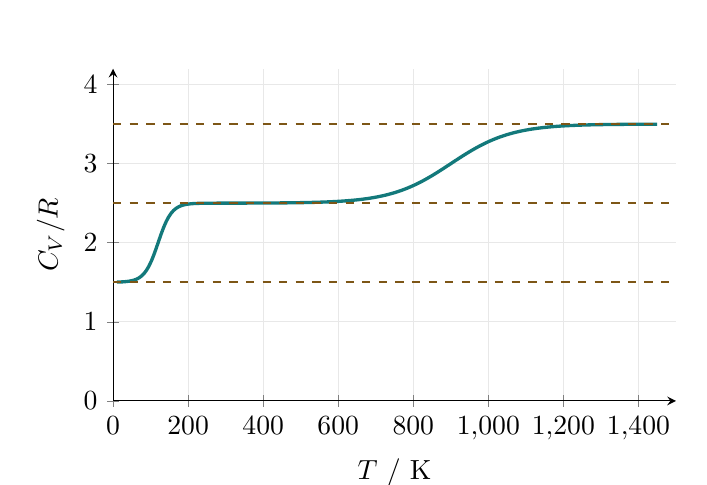
\begin{tikzpicture}
\begin{axis}[width=.72\textwidth,height=5.8cm,
xlabel={$T$ / K},ylabel={$C_V/R$},
xmin=0,xmax=1500,ymin=0,ymax=4.2,
grid=major,grid style={gray!18},
axis lines=left]
\addplot[sea,very thick,domain=10:1450,samples=220]
{1.5 + 1/(1+exp(-(x-120)/18)) + 1/(1+exp(-(x-900)/80))};
\addplot[gold!80!black,dashed,thick] coordinates {(0,1.5) (1500,1.5)};
\addplot[gold!80!black,dashed,thick] coordinates {(0,2.5) (1500,2.5)};
\addplot[gold!80!black,dashed,thick] coordinates {(0,3.5) (1500,3.5)};
\end{axis}
\end{tikzpicture}
\captionof{figure}{双原子分子定容热容随温度变化的典型趋势示意。}
\end{center}

\begin{notebox}
注意：实验上不同温度下的热容并不总是严格等于经典理论给出的常数，这正是量子效应的重要迹象。低温下某些自由度“冻住”，不能简单使用经典能量均分定理。
\end{notebox}

\section{统计规律的初步讨论}
前面已从物理应用引入了 Maxwell--Boltzmann 的指数权重。本节将从能级占据与简并度出发，逐项比较三种体系的组态计数，并给出平衡分布的极值推导。

\subsection*{简并度 $g_i$ 与三种系统的微观状态计数}
令第 $i$ 个单粒子能级为 $\varepsilon_i$，它含有 $g_i$ 个\textbf{不同的单粒子量子态}（简并度），该能级上有 $N_i$ 个粒子。满足
\[
\sum_iN_i=N,\qquad \sum_iN_i\varepsilon_i=E.
\]
必须区分能级与量子态：一个能级可能对应多个量子态；占据数 $N_i$ 指整个能级上的粒子总数。

\paragraph{（一）Boltzmann 系统}
先按可区分粒子的经典模型计数。把 $N$ 个可标记粒子分配到能级，选出各组的组合数为
\[
\frac{N!}{\prod_iN_i!}.
\]
每个占据第 $i$ 能级的粒子均有 $g_i$ 种量子态选择，因此
\[
\boxed{\Omega_{\rm B}
=\frac{N!}{\prod_iN_i!}\prod_i g_i^{N_i}.}
\]
取对数并使用 Stirling 近似，
\[
\ln\Omega_{\rm B}\simeq \ln N!-\sum_i\ln N_i!
+\sum_iN_i\ln g_i.
\]
令 $\mathcal L=\ln\Omega-\alpha\sum_iN_i-\beta\sum_iN_i\varepsilon_i$，
对每个 $N_i$ 求极值：
\[
-\ln N_i+\ln g_i-\alpha-\beta\varepsilon_i=0.
\]
于是
\[
\boxed{N_i=g_i e^{-\alpha-\beta\varepsilon_i}},\qquad
\beta=\frac1{\kb T}.
\]
更规范的经典相同粒子统计需考虑 Gibbs 的 $1/N!$ 修正，但不改变此处能级相对占据数的分布形式。

\paragraph{（二）Bose 系统}
玻色子不可分辨，一个量子态可以容纳任意多个玻色子。把 $N_i$ 个相同粒子放入 $g_i$ 个不同态，相当于寻找非负整数解
$n_1+\cdots+n_{g_i}=N_i$。利用插板法：
\[
\boxed{\Omega_{{\rm BE},i}
=\binom{N_i+g_i-1}{N_i}
=\frac{(N_i+g_i-1)!}{N_i!(g_i-1)!}.}
\]
各能级的组态数相乘：
\[
\boxed{\Omega_{\rm BE}=\prod_i
\frac{(N_i+g_i-1)!}{N_i!(g_i-1)!}.}
\]
当 $N_i,g_i$ 充分大，可用 Stirling 公式，把 $-1$ 的有限尺寸修正略去。对
$\ln\Omega_{\rm BE}-\alpha\sum_iN_i-\beta\sum_iN_i\varepsilon_i$
求驻值：
\[
\ln\frac{N_i+g_i}{N_i}=\alpha+\beta\varepsilon_i,
\]
所以
\[
\boxed{N_i^{\rm BE}
=\frac{g_i}{e^{\alpha+\beta\varepsilon_i}-1}.}
\]

\paragraph{（三）Fermi 系统}
费米子遵守 Pauli 不相容原理，每个\emph{单粒子量子态}至多占一个粒子，因此 $0\le N_i\le g_i$。从 $g_i$ 个态中挑选 $N_i$ 个：
\[
\boxed{\Omega_{{\rm FD},i}=\binom{g_i}{N_i}
=\frac{g_i!}{N_i!(g_i-N_i)!}.}
\]
总组态数是各能级计数的乘积，作同样的约束极大化，
\[
\ln\frac{g_i-N_i}{N_i}=\alpha+\beta\varepsilon_i,
\]
得到
\[
\boxed{N_i^{\rm FD}
=\frac{g_i}{e^{\alpha+\beta\varepsilon_i}+1}.}
\]
三种体系可以统一写成如下对照：
\[
\begin{array}{c|c}
\text{统计}& \text{能级平均占据数}\\\hline
\mathrm{MB}&g_i e^{-(\varepsilon_i-\mu)/\kb T}\\
\mathrm{BE}&g_i/[e^{(\varepsilon_i-\mu)/\kb T}-1]\\
\mathrm{FD}&g_i/[e^{(\varepsilon_i-\mu)/\kb T}+1]
\end{array}
\]
其中 $\alpha=-\mu/(\kb T)$。若指数因子 $e^{(\varepsilon_i-\mu)/\kb T}\gg1$，玻色和费米两式均趋于经典 Boltzmann 形式。

\begin{examplebox}
设一个能级有 $g_i=4$ 个不同单粒子态，放入 $N_i=2$ 个粒子。若按上述经典可标记粒子、玻色粒子、费米粒子的态内计数，分别为
$4^2=16$、$\binom{5}{2}=10$、$\binom{4}{2}=6$。
这个小例子直观说明三种统计的差异来自\textbf{不可分辨性和占据限制}。
\end{examplebox}
\begin{notebox}
需要注意：把 $g_i$ 引入三种计数时，$g_i$ 是一个能级包含的\emph{可区别单粒子态数}，不是粒子数；若 $N_i$ 表示整个能级上的占据数，BE/FD 的分子必须有 $g_i$。对某个单一量子态的平均占据数才没有 $g_i$ 因子。
\end{notebox}

%===========================
\chapter{近平衡态中的输运过程}

\section{输运现象及其宏观规律}
处于平衡态的系统，宏观量在空间上均匀，不存在净流。当系统略微偏离平衡态时，各种不均匀性会在微观随机运动的作用下逐渐被抹平，这就是输运过程。最常见的有三类：

\subsection*{1. 扩散}
当粒子数密度 $n$ 在空间上不均匀时，会出现粒子从高密度区域向低密度区域的净迁移。Fick 定律写成
\[
\boxed{\bm j_n=-D\nabla n},
\]
其中 $\bm j_n$ 是粒子数流密度，$D$ 是扩散系数。

\subsection*{2. 热传导}
当温度分布不均匀时，热量将自发地从高温处流向低温处。Fourier 定律写成
\[
\boxed{\bm j_Q=-\kappa \nabla T},
\]
其中 $\bm j_Q$ 是热流密度，$\kappa$ 是热导率。

\subsection*{3. 黏滞}
流体各处速度不同，会因分子交换动量而产生内摩擦效应。对于沿 $x$ 方向流动、速度沿 $y$ 方向变化的简单剪切流，
\[
\boxed{\tau_{xy}=\eta \pp{u_x}{y}},
\]
其中 $\eta$ 是黏滞系数，$\tau_{xy}$ 表示单位面积上的切向应力。

\begin{center}
\begin{tikzpicture}[>=Latex]
\draw[thick] (0,0) rectangle (8,3.2);
\foreach \y/\len in {0.45/1.8,0.95/2.5,1.45/3.3,1.95/4.3,2.45/5.6,2.95/6.8}
  \draw[->,sea,thick] (0.6,\y) -- ++(\len,0);
\node[right] at (7.8,2.95) {$u=u(y)$};
\node[above] at (4.0,3.2) {速度梯度导致黏滞应力};
\draw[->] (8.6,0.2)--(8.6,3.1) node[above] {$y$};
\end{tikzpicture}
\end{center}


\subsection*{题目：内部均匀产热的球体}
问：为什么温度高于 \(\SI{37}{\celsius}\) 的体内环境可能仍有益于热量向外散出？其简化模型是半径 $R$、热导率 $\kappa$ 恒定且\textbf{内部单位体积均匀产热} $a$ 的球体，表面温度固定为 $T_0$。不应把它替换成没有体积热源的球壳问题。

半径 $r$ 以内的总产热功率为
\[
\dot Q_{\rm gen}(r)=a\frac{4\pi r^3}{3}.
\]
稳态能量守恒要求它恰好等于穿过半径 $r$ 球面的向外热流功率，结合 Fourier 定律：
\[
a\frac{4\pi r^3}{3}=-4\pi r^2\kappa\frac{\dd T}{\dd r}.
\]
约去共同因子，得到
\[
\frac{\dd T}{\dd r}=-\frac{a}{3\kappa}r,\quad
T(r)=-\frac{a}{6\kappa}r^2+C.
\]
代入边界条件 $T(R)=T_0$：
\[
\boxed{T(r)=T_0+\frac{a}{6\kappa}(R^2-r^2).}
\]
因此中心温度 $T(0)=T_0+aR^2/(6\kappa)$ 高于表面，中心处由于对称性温度梯度为零。这是\emph{均匀体积产热}造成的温度分布；无源球壳稳态结果 $T=C_1+C_2/r$ 不能直接用于本题。

\begin{center}
\begin{tikzpicture}[>=Latex]
\shade[inner color=gold!38,outer color=sea!12] (0,0) circle(1.7);
\draw[ink,thick] (0,0) circle(1.7);
\draw[->,sea,thick] (0,0)--(1.7,0) node[midway,above] {$r$};
\draw[->,gold,thick] (1.1,1.1)--(1.85,1.85);
\draw[->,gold,thick] (-1.1,1.1)--(-1.85,1.85);
\node at (0,-.55){内部产热 $a$};
\node[right] at (1.72,-.8){边界 $T(R)=T_0$};
\end{tikzpicture}
\end{center}
\section{气体分子的碰撞过程及其概率分布}
讨论平均自由程、相对速度以及自由程分布。

\subsection*{平均自由程的几何估计}
若把气体分子近似看作直径为 $d$ 的硬球，则两个分子发生碰撞相当于一中心分子扫出截面积
\[
\sigma=\pi d^2
\]
的碰撞圆柱。若其他分子暂且视为静止，数密度为 $n$，则分子走过长度 $\ell$ 时，扫过体积为
\[
\sigma \ell
\]
其中平均含有 $n\sigma \ell$ 个分子，因此平均自由程量级为
\[
\lambda\sim\frac{1}{n\sigma}.
\]
更精确地考虑到所有分子都在运动，平均相对速度引入一个 $\sqrt2$ 因子，故
\[
\boxed{
\lambda=\frac{1}{\sqrt2\,n\sigma}
=\frac{1}{\sqrt2\,\pi d^2n}
}.
\]
利用 $p=n\kb T$ 还可写成
\[
\boxed{\lambda=\frac{\kb T}{\sqrt2\,\pi d^2p}}.
\]

\subsection*{相对速度分布}
若两粒子速度分别为 $\vv_1,\vv_2$，定义相对速度
\[
\vu=\vv_1-\vv_2.
\]
注意：由于两粒子的速度都服从 Maxwell 分布，因此相对速度也服从 Maxwell 型分布，只不过其中的质量应由约化质量替代。对于同种分子，最终仍可写成
\[
f(u)\propto u^2\exp\left(-\frac{mu^2}{4\kb T}\right).
\]
这使得我们能进一步计算平均相对速率。


\subsection*{相对速率积分、碰撞率与 $\sqrt2$ 因子}
对同种 Maxwell 气体的两个独立分子，速度分量均为方差 $\kb T/m$ 的正态分布。
相对速度分量 $u_x=v_{1x}-v_{2x}$ 的方差为 $2\kb T/m$，三维速率概率密度为
\[
f_u(u)=4\pi\left(\frac{m}{4\pi\kb T}\right)^{3/2}
u^2 e^{-mu^2/(4\kb T)}.
\]
计算均值：
\[
\begin{aligned}
\avg{u}
&=4\pi\left(\frac m{4\pi\kb T}\right)^{3/2}
\int_0^\infty u^3e^{-mu^2/(4\kb T)}\dd u\\
&=\sqrt{\frac{16\kb T}{\pi m}}
=\sqrt2\,\avg v.
\end{aligned}
\]
故一粒子的平均碰撞频率 $z=n\sigma\avg{u}$，平均自由时间
$\tau=1/z$，利用 $\lambda=\avg v\,\tau$ 得
\[
\boxed{\lambda=\frac{\avg v}{n\sigma\avg u}
=\frac1{\sqrt2\,n\sigma}.}
\]
这是稀薄同种硬球气体、分子碰撞不相关等假设下的公式。

\subsection*{自由程的指数分布}
设分子在走过无穷小长度 $\dd \ell$ 的过程中发生碰撞的概率正比于 $\dd \ell$：
\[
P(\text{在 }\dd\ell\text{ 内碰撞})=\frac{\dd\ell}{\lambda}.
\]
记 $P_0(\ell)$ 表示走到距离 $\ell$ 仍未碰撞的概率，则
\[
P_0(\ell+\dd\ell)=P_0(\ell)\left(1-\frac{\dd\ell}{\lambda}\right).
\]
于是
\[
\frac{\dd P_0}{\dd\ell}=-\frac{P_0}{\lambda},
\qquad P_0(0)=1.
\]
解得
\[
P_0(\ell)=e^{-\ell/\lambda}.
\]
因此首次碰撞发生在区间 $[\ell,\ell+\dd\ell]$ 的概率密度为
\[
f(\ell)\dd\ell
=
-\dd P_0(\ell)
=
\frac1\lambda e^{-\ell/\lambda}\dd\ell.
\]
所以
\[
\boxed{f(\ell)=\frac1\lambda e^{-\ell/\lambda}},\qquad \ell\ge0.
\]
并且
\[
\avg{\ell}=\int_0^\infty \ell f(\ell)\dd\ell=\lambda.
\]

\begin{notebox}
在这里实际上给出了一个非常典型的“等待时间/等待路程”的指数分布例子。它的前提是假定碰撞是独立、稀薄且均匀的，因此不适用于高密度液体或强关联系统。
\end{notebox}

\section{气体输运现象的微观解释}
利用平均自由程的思想，可以对扩散、黏滞和热传导系数给出数量级估计。

\subsection*{扩散系数}
设平均热速率为 $\bar v$，平均碰撞时间为
\[
\tau\sim \frac{\lambda}{\bar v}.
\]
在随机游走近似下，扩散系数的量级是
\[
\boxed{D\sim \frac13\bar v\lambda}.
\]

\subsection*{黏滞系数}
以简单剪切流为例，穿过某个平面的分子平均携带距该平面约一自由程处的流动动量，从而造成切向动量通量。数量级分析给出
\[
\boxed{\eta\sim \frac13\rho\bar v\lambda},
\]
其中 $\rho=nm$ 是质量密度。


\subsection*{穿越平面的黏滞动量通量积分}
设流速沿 $x$ 方向而沿 $z$ 方向变化，分子撞过面积 $A$ 的平面时，出发位置相对平面约为 $-\ell\cos\theta$。Taylor 展开
\[
u_x(z-\ell\cos\theta)\simeq
u_x(z)-\ell\cos\theta\,\frac{\dd u_x}{\dd z}.
\]
按照各向同性的入射角分布，上下两侧动量通量差包含角平均
\[
\int_0^{\pi/2}\cos^2\theta\sin\theta\,\dd\theta=\frac13.
\]
于是得到模型量级
\[
\tau_{xz}\simeq
-\frac13 nm\avg{v\ell}\frac{\dd u_x}{\dd z}
\simeq-\frac13\rho\bar v\lambda\frac{\dd u_x}{\dd z},
\]
这里负号指\emph{从上向下传递的 $x$ 向动量通量}与速度梯度相反；若采用作用于上表面的应力张量分量定义，则常写为
$\tau_{xz}=\eta\,\dd u_x/\dd z$。约定必须在图中明确。
由此
\[
\eta\simeq\frac13\rho\bar v\lambda,\quad
\kappa\simeq\frac13c_V^{(\rm vol)}\bar v\lambda,\quad
D\simeq\frac13\bar v\lambda.
\]
中 $\eta\propto T^{1/2}$ 是这一模型的温标结果，并非所有实际气体的精确幂律。


\subsection*{热导率}
若单位体积定容热容记为 $c_V^{(\mathrm{vol})}$，则热导率量级为
\[
\boxed{\kappa\sim \frac13c_V^{(\mathrm{vol})}\bar v\lambda}.
\]

\begin{keybox}
三种输运系数有着完全类似的结构：
\[
D\sim \frac13\bar v\lambda,\qquad
\eta\sim \frac13\rho\bar v\lambda,\qquad
\kappa\sim \frac13c_V^{(\mathrm{vol})}\bar v\lambda.
\]
它们都可以理解为“某种宏观量被分子热运动跨越一自由程携带”的结果。
\end{keybox}

\begin{notebox}
还可以指出：对稀薄气体，简单模型预言黏滞系数与压强几乎无关，而与温度大致呈幂律关系。更精确的指数需借助更完整的碰撞理论，简单平均自由程模型只能给出量级与趋势。
\end{notebox}

\section{布朗运动及其引起的扩散}
先讨论随机游走，再引入 Langevin 方程，并最后与 RC 电路热噪声类比。

\subsection*{随机游走图像}
设布朗粒子每经过时间 $\tau$ 发生一次无规则位移，位移长度尺度为 $\lambda$，方向各向同性。经过 $n$ 步后，总位移是
\[
\vr=\vr_1+\vr_2+\cdots+\vr_n.
\]
由于各步独立、方向无偏，
\[
\avg{\vr}=0,
\qquad
\avg{r^2}=n\lambda^2.
\]
又因为总时间
\[
t=n\tau,
\]
故
\[
\avg{r^2}\propto t.
\]
这正是扩散规律的微观来源。

\subsection*{Langevin 方程}
把布朗粒子的运动写为
\[
m\frac{\dd v}{\dd t}=-\zeta v+\xi(t),
\]
其中
\begin{itemize}[leftmargin=2.2em]
\item $-\zeta v$ 表示黏滞阻力；
\item $\xi(t)$ 表示周围分子碰撞产生的随机力。
\end{itemize}
设
\[
\avg{\xi(t)}=0,
\qquad
\avg{\xi(t)\xi(t')}=2\zeta\kb T\,\delta(t-t').
\]
将方程写成
\[
\frac{\dd v}{\dd t}+\gamma v=f(t),
\qquad
\gamma=\frac{\zeta}{m},\quad f(t)=\frac{\xi(t)}{m}.
\]
乘以积分因子 $\ee^{\gamma t}$ 可得
\[
v(t)=v_0e^{-\gamma t}+\int_0^t e^{-\gamma(t-s)}f(s)\dd s.
\]
由此可算出
\[
\avg{v(t)}=\avg{v_0}\ee^{-\gamma t},
\]
并且
\[
\avg{v^2(t)}
=
\avg{v_0^2}\ee^{-2\gamma t}
+\frac{\kb T}{m}\left(1-\ee^{-2\gamma t}\right).
\]
$t\to\infty$ 时，
\[
\avg{v^2}\to \frac{\kb T}{m},
\]
与一维能量均分定理一致：
\[
\frac12m\avg{v^2}=\frac12\kb T.
\]


\subsection*{随机力关联与二阶矩的完整计算}
为与的记号一致，设
\[
\gamma=\zeta/m,\qquad f(t)=\xi(t)/m,\qquad
\avg{f(t)}=0,\qquad\avg{f(t_1)f(t_2)}=A\delta(t_1-t_2).
\]
所谓白噪声并不是每一时刻取值都为普通意义的有限随机数，而是一个短相关时间噪声的理想化极限；这里仅使用 Dirac $\delta$ 的积分筛选性质
$\int \delta(t-t_0)h(t)\dd t=h(t_0)$。
初始速度与 $t>0$ 的随机力假定不相关。

代入积分解，
\[
v(t)=v_0e^{-\gamma t}+
\int_0^t e^{-\gamma(t-s)}f(s)\dd s,
\]
平方并取平均时需要\textbf{保留两个随机积分的交叉项}：
\begin{align*}
\avg{v^2(t)}
&=\avg{v_0^2}e^{-2\gamma t}
+2e^{-\gamma t}\int_0^t e^{-\gamma(t-s)}
\avg{v_0f(s)}\dd s\\
&\quad+\int_0^t\!\int_0^t e^{-\gamma(2t-s-s')}
\avg{f(s)f(s')}\dd s\,\dd s'.
\end{align*}
中间项在上述独立性假设下为零。对双重积分应用相关函数：
\[
\begin{aligned}
I&=A\int_0^t\!\int_0^t
e^{-\gamma(2t-s-s')}\delta(s-s')\dd s'\dd s\\
&=A\int_0^t e^{-2\gamma(t-s)}\dd s
=\frac{A}{2\gamma}(1-e^{-2\gamma t}).
\end{aligned}
\]
从而
\[
\boxed{\avg{v^2(t)}
=\avg{v_0^2}e^{-2\gamma t}
+\frac{A}{2\gamma}(1-e^{-2\gamma t}).}
\]
令 $t\to\infty$ 并利用一维能量均分
$m\avg{v^2}/2=\kb T/2$，可反推出
\[
\frac{A}{2\gamma}=\frac{\kb T}{m},\qquad
\boxed{A=\frac{2\gamma\kb T}{m}.}
\]
这就是阻尼与随机力强度之间的涨落--耗散关系。

\subsection*{均方位移的微分方程解法}
从 $\dot v=-\gamma v+f$ 和 $\dot x=v$ 出发，先推导
\[
\frac{\dd}{\dd t}\avg{x^2}=2\avg{xv}.
\]
对 $\avg{xv}$ 求导（加性理想白噪声，使用恰当的随机积分解释）：
\[
\frac{\dd}{\dd t}\avg{xv}=
\avg{v^2}-\gamma\avg{xv}.
\]
若速度分布已经达到平衡，则 $\avg{v^2}=\kb T/m$，因此
\[
\frac12\frac{\dd^2}{\dd t^2}\avg{\Delta x^2}
+\frac{\gamma}{2}\frac{\dd}{\dd t}\avg{\Delta x^2}
=\frac{\kb T}{m}.
\]
设初始位移为零且 $\avg{\Delta x\,v}(0)=0$，解得
\[
\boxed{\avg{\Delta x^2(t)}
=\frac{2\kb T}{m\gamma}
\left[t-\frac{1-e^{-\gamma t}}{\gamma}\right].}
\]
$t\ll\gamma^{-1}$ 时作指数展开，得到弹道运动
\[
\avg{\Delta x^2}\simeq \frac{\kb T}{m}t^2;
\]
$t\gg\gamma^{-1}$ 时得到普通扩散规律
\[
\avg{\Delta x^2}\simeq 2Dt,\qquad
\boxed{D=\frac{\kb T}{m\gamma}=\frac{\kb T}{\zeta}.}
\]
因而所强调的 $\avg{x^2}\propto t$ 仅是\textbf{长时间极限}，短时间不是这个规律。
\begin{notebox}
校订：推导中 $\delta(t_1-t_2)$ 表示两个\emph{时间变量}之间的相关，不应直接写成“不同时间的随机力乘积为零”，而是说不同时间点的相关函数在理想白噪声模型中仅在时间相同处具有 $\delta$ 支持。阻尼记号 $\gamma=\zeta/m$ 和单粒子速率等其它参数不可混用。
\end{notebox}

\subsection*{Einstein 扩散公式}
把速度再对时间积分得位移，最终得到长时间极限下
\[
\avg{[x(t)-x(0)]^2}\simeq 2Dt,
\]
其中
\[
\boxed{D=\frac{\kb T}{\zeta}}.
\]
三维情况下
\[
\boxed{\avg{|\vr(t)-\vr(0)|^2}=6Dt}.
\]
若布朗粒子是半径为 $a$ 的小球，在黏度为 $\eta$ 的流体中满足 Stokes 阻力
\[
\zeta=6\pi\eta a,
\]
则得到著名的 Stokes--Einstein 关系：
\[
\boxed{D=\frac{\kb T}{6\pi\eta a}}.
\]

\subsection*{RC 电路的类比}
RC 电路也可以说明热噪声问题。设电容器带电量为 $q$，则回路方程可写为
\[
R\frac{\dd q}{\dd t}+\frac{q}{C}=\mathcal E(t),
\]
其中 $\mathcal E(t)$ 是热噪声电动势。它与 Langevin 方程在数学形式上完全类似。平衡时
\[
\frac{\avg{q^2}}{2C}=\frac12\kb T,
\]
故
\[
\avg{q^2}=C\kb T.
\]
这对应电容器上的热涨落。


\subsection*{RC 热噪声的参数对应与均方值}
对无外加驱动的串联 RC 回路，电阻热噪声等效为随机电动势 $\mathcal E(t)$，电荷满足
\[
R\dot q+\frac qC=\mathcal E(t).
\]
与 $\dot v=-\gamma v+f(t)$ 对照，可取
\[
\gamma=\frac1{RC},\qquad f_q(t)=\frac{\mathcal E(t)}R.
\]
平衡时电容能量 $U_C=q^2/(2C)$ 的经典能量均分给出
\[
\frac{\avg{q^2}}{2C}=\frac12\kb T
\Longrightarrow
\boxed{\avg{q^2}=C\kb T,\quad
\avg{V_C^2}=\frac{\kb T}C}.
\]
采用单边频谱密度（$f\ge0$）时，Johnson--Nyquist 关系写为
$S_{\mathcal E}(f)=4\kb TR$，单位 $\mathrm{V^2\,Hz^{-1}}$；
RC 滤波后输出的电压方差
\[
\avg{V_C^2}=
\int_0^\infty
\frac{4\kb TR}{1+(2\pi fRC)^2}\dd f
=\frac{\kb T}{C}.
\]
这里的积分可用 $u=2\pi fRC$，并利用
$\int_0^\infty (1+u^2)^{-1}\dd u=\pi/2$ 计算。


%===========================
\chapter{热力学第一定律}

\section{热力学第一定律}
热力学第一定律本质上是能量守恒定律在热现象中的表达。

\subsection*{功与热}
功 $W$ 和热量 $Q$ 都是\textbf{过程量}，不是状态量。本讲义采用与一致的符号约定：\textbf{系统吸热为正，系统对外做功为正}。于是
\[
\boxed{\Delta U=Q-W},
\]
或微分形式
\[
\boxed{\dd U=\delta Q-\delta W}.
\]
其中 $U$ 是系统内能，是状态量。

对于准静态体积功，
\[
\delta W=p\dd V.
\]
于是
\[
\dd U=\delta Q-p\dd V.
\]

\begin{notebox}
画出了两个不同路径连接同一始末态的 $p$-$V$ 图，用来说明功是路径相关的。即使初态与末态相同，不同过程做功一般不同；但内能变化只取决于始末态。
\end{notebox}

\section{热力学第一定律对理想气体的应用}
重点讨论四种典型过程和多方过程。

\subsection*{理想气体内能只与温度有关}
对理想气体，
\[
U=U(T),
\qquad \dd U=C_V\dd T.
\]
这使得求解各种过程大大简化。

\subsection*{（一）等温过程}
若
\[
T=\const,
\]
则理想气体内能不变：
\[
\Delta U=0.
\]
可逆等温过程中
\[
W=\int_{V_1}^{V_2}p\dd V
=
\int_{V_1}^{V_2}\frac{\nu RT}{V}\dd V
=
\nu RT\ln\frac{V_2}{V_1}.
\]
由第一定律，
\[
Q=W.
\]

\subsection*{（二）等压过程}
若
\[
p=\const,
\]
则
\[
W=p(V_2-V_1).
\]
又因
\[
\Delta U=C_V(T_2-T_1),
\]
并用理想气体方程
\[
p(V_2-V_1)=\nu R(T_2-T_1),
\]
故
\[
Q=\Delta U+W=(C_V+\nu R)(T_2-T_1).
\]
于是
\[
\boxed{C_p=C_V+\nu R}.
\]

\subsection*{（三）等容过程}
若
\[
V=\const,
\]
则
\[
W=0,
\qquad
Q=\Delta U=C_V(T_2-T_1).
\]

\subsection*{（四）可逆绝热过程}
若
\[
\delta Q=0,
\]
则
\[
\dd U=-p\dd V.
\]
对理想气体
\[
C_V\dd T=-p\dd V=-\frac{\nu RT}{V}\dd V.
\]
整理得
\[
C_V\frac{\dd T}{T}=-\nu R\frac{\dd V}{V}.
\]
积分可得
\[
TV^{\gamma-1}=\const,
\qquad
\gamma=\frac{C_p}{C_V}.
\]
再与理想气体方程联立，可得
\[
\boxed{pV^\gamma=\const}.
\]
这是绝热过程中的重要推导结果。

\begin{center}
\begin{tikzpicture}
\begin{axis}[width=.82\textwidth,height=6cm,
xlabel={$V$},ylabel={$p$},
xmin=.6,xmax=4.2,ymin=0,ymax=4.2,
xtick=\empty,ytick=\empty,axis lines=left]
\addplot[sea,very thick,domain=.9:4,samples=160]{2.8/x};
\addplot[gold!85!black,very thick,domain=.9:4,samples=160]{2.8/x^1.4};
\node[sea] at (axis cs:2.85,1.35) {等温};
\node[gold!85!black] at (axis cs:2.55,0.8) {可逆绝热};
\end{axis}
\end{tikzpicture}
\captionof{figure}{同一初态出发，绝热线比等温线更陡。}
\end{center}



\begin{figure}[htbp]\centering
\begin{tikzpicture}[>=Latex,scale=.82]
\draw[ink,thick] (-1.6,-.5) .. controls (-2.4,.8) and (-1.4,1.6) .. (-.55,1.6) --(-.55,4.6);
\draw[ink,thick] (1.6,-.5) .. controls (2.4,.8) and (1.4,1.6) .. (.55,1.6) --(.55,4.6);
\draw[ink,thick] (-1.6,-.5) arc[start angle=180,end angle=360,x radius=1.6,y radius=.55];
\fill[sea!25] (-.52,3.0) rectangle (.52,3.28);
\draw[ink,thick] (-.52,3.0) rectangle (.52,3.28);
\draw[->,sea,thick] (0,3.3)--(0,4.0) node[right] {$pA$};
\draw[->,gold!85!black,thick] (0,2.98)--(0,2.2) node[right] {$mg$};
\draw[->,ink,thick] (-.8,3.8)--(-.8,3.28) node[left] {$p_0A$};
\node[right] at (1.3,3.15) {小球 $m$};
\node[right] at (1.6,.4) {气体 $p,V$};
\end{tikzpicture}
\caption{Rüchardt 振动法：由气室、竖直导管和可动小球组成的振动系统。}
\end{figure}

\subsection*{Rüchardt 气体振动法测 $\gamma$}
画出由细长竖直管、活塞（或小球）和气室构成的装置。设气室平衡体积 $V$、内压 $p$，可动部分有效截面积 $A$、质量 $m$，上方外压 $p_{\rm ext}$，平衡条件是
\[
pA=p_{\rm ext}A+mg.
\]
从平衡位置向上微移 $x$，气体体积改变 $\Delta V=Ax$，假设振动快到与环境交换热量可忽略，并且气室中的过程可以看成\textbf{小振幅可逆绝热}：
\[
pV^\gamma=\const,\qquad
\frac{\dd p}{\dd V}=-\frac{\gamma p}{V}.
\]
因此压强变化 $\Delta p\simeq-\gamma p Ax/V$，对活塞的恢复力为
\[
F=A\Delta p=-\frac{\gamma pA^2}{V}x.
\]
牛顿第二定律化为
\[
m\ddot x+\frac{\gamma pA^2}{V}x=0.
\]
这是简谐运动，角频率与周期分别为
\[
\omega^2=\frac{\gamma pA^2}{mV},\qquad
\boxed{\gamma=\frac{4\pi^2mV}{pA^2\tau^2}}.
\]
在实际测量中应考虑管壁摩擦、泄漏和非绝热损失。以下在旧版中遗漏了，现恢复完整力学推导。

\subsection*{干绝热大气温度直减率}
设一团空气快速上升，近似绝热，且上升过程中其压强保持与外界静力平衡压强一致。对定比热的理想气体
\[
T p^{(1-\gamma)/\gamma}=\const
\quad\Longrightarrow\quad
\frac{\dd T}{T}=\frac{\gamma-1}{\gamma}\frac{\dd p}{p}.
\]
静力平衡满足
\[
\frac{\dd p}{\dd z}=-\rho g,\qquad
p=\rho R_sT,
\]
其中 $R_s$ 为单位质量气体常数，$c_p=\gamma R_s/(\gamma-1)$。
联立即得
\[
\boxed{\frac{\dd T}{\dd z}
=-\frac{\gamma-1}{\gamma}\frac g{R_s}
=-\frac g{c_p}.}
\]
对干燥空气近似 $g/c_p\simeq9.8\ {\rm K\,km^{-1}}$，将其与实际大气的直减率作了比较。两者不同，因为真实大气含水汽凝结和辐射交换，并非处处都沿可逆干绝热过程变化。


\subsection*{（五）多方过程}
最后讨论了多方过程
\[
\boxed{pV^n=\const},
\]
其中 $n$ 为多方指数。对 $n\neq1$，
\[
W=\int_{V_1}^{V_2}p\dd V
=
\frac{p_2V_2-p_1V_1}{1-n}
=
\frac{\nu R(T_2-T_1)}{1-n}.
\]
于是
\[
Q=\Delta U+W
=
\left(C_V+\frac{\nu R}{1-n}\right)(T_2-T_1).
\]
该过程中相应的热容可写作
\[
C_n=C_V+\frac{\nu R}{1-n}
=
C_V\frac{\gamma-n}{1-n}.
\]

\section{节流过程与自由膨胀}


\subsection*{焓与节流过程}
定义焓
\[
\boxed{H=U+pV}.
\]
对封闭、简单可压缩系统，结合
\[
\dd U=\delta Q-p\dd V
\]
与可逆热力学关系，可得
\[
\dd H=T\dd S+V\dd p.
\]
主要关心\textbf{节流过程}：气体通过多孔塞或狭窄阀门时，若过程稳态、绝热、且忽略进出口动能势能变化，则可证明单位质量焓近似不变，即
\[
\boxed{H_1=H_2}.
\]
Joule--Thomson 系数定义为
\[
\mu_{\mathrm{JT}}=
\left(\pp Tp\right)_H.
\]

由
\[
\dd H=C_p\dd T+\left[V-T\left(\pp VT\right)_p\right]\dd p
\]
可得
\[
\boxed{
\mu_{\mathrm{JT}}
=
\frac{T(\partial V/\partial T)_p-V}{C_p}
=
\frac{V}{C_p}(\alpha T-1)
}.
\]
对于理想气体，$\alpha=1/T$，故
\[
\mu_{\mathrm{JT}}=0.
\]
即理想气体在节流中温度不变。

\subsection*{自由膨胀}
最后讨论了气体向真空的自由膨胀。其特征是：
\[
Q=0,\qquad W=0.
\]
因此
\[
\Delta U=0.
\]
对理想气体，由于内能只与温度有关，可得
\[
\Delta T=0.
\]
但\textbf{自由膨胀是不可逆过程}，不能使用
\[
pV^\gamma=\const
\]
来描述中间路径。

\section{循环过程与 Carnot 循环}
循环过程完成一周后系统回到初态，因此
\[
\Delta U=0.
\]
故一整个循环中
\[
W_{\mathrm{net}}=Q_{\mathrm{net}}.
\]

\subsection*{热机效率}
热机从高温热源吸热 $Q_h$，向低温热源放热 $Q_c$，并对外做功 $W$。效率定义为
\[
\boxed{\eta=\frac{W}{Q_h}=1-\frac{Q_c}{Q_h}}.
\]

\subsection*{Carnot 循环}
Carnot 循环由两条等温线和两条绝热线组成。设高温热源温度为 $T_h$，低温热源温度为 $T_c$。

高温等温膨胀：
\[
Q_h=\nu RT_h\ln\frac{V_B}{V_A}.
\]
低温等温压缩：
\[
Q_c=\nu RT_c\ln\frac{V_C}{V_D}.
\]
而绝热过程满足
\[
T_hV_B^{\gamma-1}=T_cV_C^{\gamma-1},
\qquad
T_hV_A^{\gamma-1}=T_cV_D^{\gamma-1}.
\]
两式相除得
\[
\frac{V_B}{V_A}=\frac{V_C}{V_D}.
\]
所以
\[
\frac{Q_c}{Q_h}=\frac{T_c}{T_h},
\]
从而
\[
\boxed{\eta_{\mathrm{Carnot}}=1-\frac{T_c}{T_h}}.
\]

\begin{keybox}
Carnot 循环给出：在两个给定热源之间工作的任何热机，其效率都不能超过可逆 Carnot 热机的效率。这个结论将在下一章由热力学第二定律严格说明。
\end{keybox}

%===========================
\chapter{热力学第二定律}

\section{热力学第二定律的两种语言表述}
热力学第二定律的两个经典表述是：

\paragraph{Clausius 表述}
\textbf{不可能把热量从低温物体传到高温物体而不引起其他变化。}

\paragraph{Kelvin 表述}
\textbf{不可能从单一热源吸收热量并把它完全转换为功，而不引起其他变化。}

给出了两者等价的说明：如果其中一种表述被违反，就可以构造装置违反另一种表述。

\begin{notebox}
第二定律不是能量守恒定律的简单重复。第一定律只告诉我们“能量总量守恒”，而第二定律进一步限定了热量与功之间相互转化的方向性和限度。
\end{notebox}


\subsection*{两个表述等价性的双向反证}
\textbf{假设 Kelvin--Planck 表述不成立。}
存在一台循环装置 $K$，从温度 $T_h$ 的\emph{单一热源}吸收 $Q>0$，将其全部转化为功 $W=Q$，且无其他效果。
再取一台正常运行的冰箱 $R$，消耗功 $W_R>0$，从冷源吸收 $Q_c>0$，
向热源放出 $Q_c+W_R$。适当调节循环次数使 $K$ 输出的功恰好等于 $W_R$。
把 $K$ 与 $R$ 看作整体后：
\[
W_{\rm net}=0,\qquad Q_{h,\rm net}=-W_R+(Q_c+W_R)=Q_c.
\]
组合装置的唯一效果是从冷源取走 $Q_c$ 并送入热源 $Q_c$，
没有外界做功。这与 Clausius 表述矛盾。因此 Clausius 表述成立时 Kelvin--Planck 表述也必须成立。

\textbf{反过来，假设 Clausius 表述不成立。}
存在一台装置 $C$，无需外界做功便把热量 $Q_c$ 从冷源送到热源。
另取一台普通循环热机 $E$，从热源吸热 $Q_h$，向冷源排出 $Q_c$，
输出功
\[
W=Q_h-Q_c>0.
\]
将 $C$ 与 $E$ 组合，两个装置对冷源的热交换恰好相互抵消。
整个组合装置只从\emph{单一的热源}净吸收
$Q_h-Q_c=W$ 并全部输出为功，不产生其他净效果。
这便违反 Kelvin--Planck 表述。
\begin{keybox}
两条逻辑分别说明
\[
\neg K\Rightarrow\neg C,\qquad
\neg C\Rightarrow\neg K.
\]
由反证可知，两种表述对一切循环设备施加的是同一个方向性约束。
\end{keybox}
\begin{center}
\begin{tikzpicture}[>=Latex,thick]
\node[draw=sea,fill=soft,rounded corners=3pt,minimum width=3cm,minimum height=.9cm] (h) at (0,2.8){高温热源 $T_h$};
\node[draw=ink,fill=white,rounded corners=3pt,minimum width=3cm,minimum height=.9cm] (eng) at (0,1.35){组合装置};
\node[draw=gold!85!black,fill=warm,rounded corners=3pt,minimum width=3cm,minimum height=.9cm] (c) at (0,-.1){低温热源 $T_c$};
\draw[->,sea,very thick] (-.65,2.35)--(-.65,1.85) node[midway,left] {$Q_h$};
\draw[->,gold!80!black,very thick] (.65,.85)--(.65,.35) node[midway,right] {$Q_c$};
\draw[->,ink,very thick] (1.5,1.35)--(4.2,1.35) node[right] {$W$};
\node[font=\small,align=left] at (4.2,2.5) {热机和逆向搬运热量装置\\组合后抵消部分能量流};
\end{tikzpicture}
\end{center}

\section{热力学第二定律的数学表达}
先引入熵，然后给出 Clausius 不等式。

\subsection*{熵的定义}
对一个可逆过程，定义系统熵变
\[
\boxed{\dd S=\frac{\delta Q_{\rev}}{T}}.
\]
这里 $S$ 是状态量，因此系统从一个平衡态到另一个平衡态的熵变与所选可逆路径无关。

对一定量理想气体，
\[
\delta Q_{\rev}=C_V\dd T+p\dd V
=C_V\dd T+\frac{\nu RT}{V}\dd V.
\]
两边除以 $T$ 得
\[
\dd S=C_V\frac{\dd T}{T}+\nu R\frac{\dd V}{V}.
\]
积分得到
\[
\boxed{
\Delta S=C_V\ln\frac{T_2}{T_1}
+\nu R\ln\frac{V_2}{V_1}
}
\]
也可写成
\[
\boxed{
\Delta S=C_p\ln\frac{T_2}{T_1}
-\nu R\ln\frac{p_2}{p_1}
}.
\]

\subsection*{Clausius 不等式}
任意循环都满足
\[
\boxed{\oint \frac{\delta Q}{T}\le0}.
\]
其中等号对应可逆循环，小于号对应不可逆循环。

由此可得，对于任意实际过程，
\[
\Delta S\ge \int \frac{\delta Q}{T}.
\]
特别地，对于孤立系统，
\[
\boxed{\Delta S\ge0}.
\]
这就是熵增原理。


\subsection*{Clausius 不等式与 Maxwell 关系的微分链条}
在系统只做可逆体积功的前提下，
\[
\delta Q_{\rm rev}=\dd U+p\dd V,\quad
\dd S=\frac{\dd U}{T}+\frac pT\dd V.
\]
对理想气体 $\dd U=C_V\dd T$ 且 $pV=\nu RT$，因此
\[
\dd S=\frac{C_V}{T}\dd T+\frac{\nu R}{V}\dd V.
\]
如果考虑一般简单可压缩平衡系统而不是理想气体，记 $U=U(T,V)$，则
\[
\dd S=\frac1T\left(\frac{\partial U}{\partial T}\right)_V\dd T
+\frac1T\left[\left(\frac{\partial U}{\partial V}\right)_T+p\right]\dd V.
\]
令 $S$ 为状态函数，其两次交叉偏导相等。结合
$F=U-TS$、$\dd F=-S\dd T-p\dd V$，
可得
\[
\boxed{\left(\frac{\partial S}{\partial V}\right)_T
=\left(\frac{\partial p}{\partial T}\right)_V},\qquad
\boxed{\left(\frac{\partial U}{\partial V}\right)_T
=T\left(\frac{\partial p}{\partial T}\right)_V-p}.
\]
这些关系适用于相应的简单可压缩平衡系统。实际气体的内能一般依赖体积；只有理想气体才满足内能仅为温度的函数。



\begin{figure}[htbp]\centering
\begin{tikzpicture}[>=Latex]
\draw[->,ink] (0,0)--(6.7,0) node[right] {$V$};
\draw[->,ink] (0,0)--(0,4.2) node[above] {$p$};
\fill[sea] (1.3,3.3) circle(2pt);
\fill[sea] (5.3,1.1) circle(2pt);
\draw[dashed,sea,thick] (1.3,3.3) .. controls (2.1,2.3) and (3.6,1.25) .. (5.3,1.1);
\node[left] at (1.3,3.3) {$(p_1,V_1)$};
\node[right] at (5.3,1.1) {$(p_2,V_2)$};
\node[align=center,sea] at (3.6,3.1) {虚线仅连接始末态\\不可视为真实准静态路径};
\end{tikzpicture}
\caption{理想气体向真空自由膨胀：实际不可逆路径不能由连续的平衡态 $p$-$V$ 曲线表示。}
\end{figure}

\subsection*{自由膨胀中的熵变}
专门讨论了自由膨胀：虽然实际过程中
\[
Q=0,
\]
但这并不意味着
\[
\Delta S=0.
\]
因为
\[
\dd S=\frac{\delta Q_{\rev}}{T}
\]
中的 $\delta Q_{\rev}$ 指的是连接同一始末态的\textbf{可逆路径}上的热量元，而不是实际不可逆路径上的热量元。

例如一定量理想气体在绝热容器中自由膨胀，若体积从 $V_1$ 增至 $V_2$，温度不变，则
\[
\Delta S=\nu R\ln\frac{V_2}{V_1}>0.
\]

\subsection*{由 Clausius 不等式导出 Carnot 效率上限}
对于任何在 $T_h,T_c$ 两热源之间工作的循环热机，
\[
\frac{Q_h}{T_h}-\frac{Q_c}{T_c}\le0.
\]
因此
\[
\frac{Q_c}{Q_h}\ge\frac{T_c}{T_h},
\]
从而
\[
\eta=1-\frac{Q_c}{Q_h}
\le 1-\frac{T_c}{T_h}.
\]
可逆情形取等号，这正是 Carnot 效率公式。



\begin{figure}[htbp]\centering
\begin{tikzpicture}[>=Latex,scale=.9]
\node[draw=sea,rounded corners,fill=soft,minimum width=3cm,minimum height=.75cm] (H) at (0,2.6) {高温热源 $T_h$};
\node[draw=ink,rounded corners,minimum width=2cm,minimum height=.7cm] (E) at (-1,1) {热机};
\node[draw=ink,rounded corners,minimum width=2cm,minimum height=.7cm] (R) at (2.2,1) {逆向热机};
\node[draw=gold!70!black,rounded corners,fill=warm,minimum width=3cm,minimum height=.75cm] (L) at (0,-.8) {低温热源 $T_c$};
\draw[->,sea,thick] (-1.25,2.2)--(-1.25,1.37) node[midway,left] {$Q_h$};
\draw[->,sea,thick] (2.2,1.37)--(2.2,2.2) node[midway,right] {$Q_h'$};
\draw[->,gold!80!black,thick] (-1,-.0)--(-1,-.43) node[midway,left] {$Q_c$};
\draw[->,gold!80!black,thick] (2.2,-.43)--(2.2,.63) node[midway,right] {$Q_c'$};
\draw[->,ink,thick] (-.0,1)--(1.2,1) node[midway,above] {$W$};
\end{tikzpicture}
\caption{Carnot 定理反证：将普通热机与逆向可逆机组合，抵消净功以比较热源交换。}
\end{figure}

\subsection*{Carnot 定理与不可逆循环的完整论证}
设一台可逆热机效率为 $\eta_{\rm rev}$，另一台声称效率
$\eta>\eta_{\rm rev}$ 的热机在相同高低温热源之间工作。把可逆热机倒转作为制冷机运行，并调整循环次数，使两机器的输出和输入功量相等。
若两机功量为同一个 $W>0$，则热机从热源吸收
$Q_h=W/\eta$；逆向可逆机向热源排出
$Q_h'=W/\eta_{\rm rev}$。在 $\eta>\eta_{\rm rev}$ 的假设下
\[
Q_h<Q_h',\qquad Q_h'-Q_h>0.
\]
两个装置合并后无净功交换，净效果却把一定热量从\emph{低温热源送向高温热源}，违反 Clausius 表述。
所以
\[
\boxed{\eta\le \eta_{\rm rev}}.
\]
再把两台\emph{可逆}热机互换角色，即得两者效率相等，因而可逆热机效率仅取决于 $T_h,T_c$ 而与工作物质无关。

对任意两热源的循环热机，以吸热为正的约定写
$Q_h>0,\ Q_\ell<0$，则
\[
\frac{Q_h}{T_h}+\frac{Q_\ell}{T_\ell}\le0,
\]
其中不可逆机取严格不等式。
当循环与多个热源交换热量，分割成足够小的热交换单元并利用可逆 Carnot 辅助机的比较，可推广为
\[
\boxed{\oint\frac{\delta Q}{T_{\rm boundary}}\le0}.
\]
\emph{热交换接触处的温度}应明确写出；不可逆有限温差传热时，不能把系统某处瞬时的非平衡温度随意代入。若系统沿一条可逆闭路，则积分等于零。定义任意平衡态 $A,B$ 之间的熵差
\[
S(B)-S(A)=\int_{A,\rm rev}^{B}\frac{\delta Q_{\rm rev}}T.
\]
若实际路径不可逆，沿实际路径和反向假想可逆路径组成循环，Clausius 不等式推出
\[
\Delta S\ge \int_{A,\rm actual}^B
\frac{\delta Q}{T_{\rm boundary}},
\]
即孤立系统熵不减。



\section{自由能与 Gibbs 函数}
在介绍熵之后，进一步引入四个常用热力学势。

\subsection*{内能的基本微分关系}
对封闭简单可压缩系统，
\[
\boxed{\dd U=T\dd S-p\dd V}.
\]
这是热力学基本关系。

\subsection*{四个热力学势}
定义
\[
H=U+pV,\qquad
F=U-TS,\qquad
G=U+pV-TS.
\]
于是它们的全微分分别为
\[
\dd U=T\dd S-p\dd V,
\]
\[
\dd H=T\dd S+V\dd p,
\]
\[
\dd F=-S\dd T-p\dd V,
\]
\[
\dd G=-S\dd T+V\dd p.
\]

\subsection*{自然变量与 Maxwell 关系}
从 $F=F(T,V)$ 可得
\[
S=-\left(\pp FT\right)_V,
\qquad
p=-\left(\pp FV\right)_T.
\]
交换二阶混合偏导得
\[
\boxed{
\left(\pp SV\right)_T
=
\left(\pp pT\right)_V
}.
\]
类似地，由其他势函数可得到一组 Maxwell 关系：
\[
\left(\pp Tp\right)_S=\left(\pp VS\right)_p,\qquad
\left(\pp TV\right)_S=-\left(\pp pS\right)_V,\qquad
\left(\pp Sp\right)_T=-\left(\pp VT\right)_p.
\]

\subsection*{自由能判据}
常用平衡判据为：

\begin{itemize}[leftmargin=2.2em]
\item 在恒温、恒容条件下，自发过程总使 Helmholtz 自由能 $F$ 减小；
\item 在恒温、恒压条件下，自发过程总使 Gibbs 自由能 $G$ 减小。
\end{itemize}

这两个结论对理解相变、化学反应和平衡条件非常重要。

\section{熵及热力学第二定律的统计意义}
从组合数和信息角度解释熵的统计意义。

\subsection*{Boltzmann 熵}
若在给定宏观约束下，系统可能对应 $\Omega$ 个等概率微观状态，则熵定义为
\[
\boxed{S=\kb\ln\Omega}.
\]
微观状态数越多，对应的熵越大。

\subsection*{Gibbs 熵}
若各微观状态概率不是等概率，而是 $p_i$，则更一般地定义
\[
\boxed{S=-\kb\sum_i p_i\ln p_i},
\qquad
\sum_i p_i=1.
\]
当所有态等概率时 $p_i=1/\Omega$，该式自然退化为
\[
S=\kb\ln\Omega.
\]

\subsection*{熵增原理的统计理解}
孤立系统为什么趋向于熵增？统计解释是：满足平衡宏观条件的微观状态数远多于远离平衡的状态数，因此系统几乎必然从“少数微观实现方式的宏观态”走向“多数微观实现方式的宏观态”。这并不是某种额外的机械力，而是大数统计规律的体现。


\subsection*{由多项式计数推出 Boltzmann 熵}
采用 $N$ 个粒子被划分为多个子类、各类占据数为 $N_i$ 的计数方式：
\[
N=\sum_iN_i,\qquad
\Omega=\frac{N!}{\prod_iN_i!}.
\]
若 $N_i$ 很大，Stirling 近似使
\[
\begin{aligned}
\ln\Omega
&=\ln N!-\sum_i\ln N_i!\\
&\simeq N\ln N-\sum_iN_i\ln N_i\\
&=-N\sum_i p_i\ln p_i,\qquad p_i=N_i/N.
\end{aligned}
\]
故对这种由\emph{可区分试验对象的宏观占据计数}构成的模型，
\[
\boxed{S\simeq-N\kb\sum_i p_i\ln p_i}.
\]
这里的 $p_i$ 是单粒子的类别概率；而一般 Gibbs 熵
$S=-\kb\sum_jP_j\ln P_j$ 中 $P_j$ 是\emph{整个系统微观状态 $j$} 的概率，
两者的求和对象不同。在独立可区分粒子的模型和适当的粗粒化约定下，它们才有上述联系。
若系统等概率占有 $\Omega$ 个微观态，便恢复 $S=\kb\ln\Omega$。
对普通物理而言，这里还应解释统计的不可逆性：宏观态的组合数相差非常巨大，
所以朝向最大组态数的变化在宏观尺度上具有极高概率，但微观动力学本身并不因此失去时间反演对称性。


\appendix
\chapter{公式速查}

\renewcommand{\arraystretch}{1.5}
\small
\noindent\begin{tabularx}{\textwidth}{@{}p{.26\textwidth}X@{}}
\toprule
主题 & 关键公式 \\
\midrule
理想气体状态方程 & $pV=\nu RT=Nk_{\mathrm B}T$ \\
压强公式 & $p=\frac13nm\avg{v^2}$ \\
温度与平均动能 & $\frac12m\avg{v^2}=\frac32\kb T$ \\
Maxwell 速率分布 &
$f_v(v)=4\pi\left(\frac{m}{2\pi\kb T}\right)^{3/2}v^2e^{-mv^2/(2\kb T)}$ \\
三种典型速率 &
$v_{\mathrm{mp}}=\sqrt{2\kb T/m},\ \avg v=\sqrt{8\kb T/(\pi m)},\ v_{\mathrm{rms}}=\sqrt{3\kb T/m}$ \\
平均自由程 &
$\lambda=1/(\sqrt2\,\pi d^2n)=\kb T/(\sqrt2\,\pi d^2p)$ \\
输运系数量级 &
$D\sim \frac13\bar v\lambda,\ \eta\sim \frac13\rho\bar v\lambda,\ \kappa\sim \frac13c_V^{(\mathrm{vol})}\bar v\lambda$ \\
热力学第一定律 & $\dd U=\delta Q-\delta W$ \\
可逆绝热过程 & $pV^\gamma=\const,\ TV^{\gamma-1}=\const$ \\
熵 & $\dd S=\delta Q_{\rev}/T$ \\
Clausius 不等式 & $\oint \delta Q/T\le0$ \\
Carnot 效率 & $\eta_{\max}=1-T_c/T_h$ \\
自由能 & $F=U-TS,\ G=U+pV-TS$ \\
Boltzmann 熵 & $S=\kb\ln\Omega$ \\
\bottomrule
\end{tabularx}


\vfill


\end{document}
